\documentclass[]{article}
\usepackage{lmodern}
\usepackage{amssymb,amsmath}
\usepackage{ifxetex,ifluatex}
\usepackage{fixltx2e} % provides \textsubscript
\ifnum 0\ifxetex 1\fi\ifluatex 1\fi=0 % if pdftex
  \usepackage[T1]{fontenc}
  \usepackage[utf8]{inputenc}
\else % if luatex or xelatex
  \ifxetex
    \usepackage{mathspec}
  \else
    \usepackage{fontspec}
  \fi
  \defaultfontfeatures{Ligatures=TeX,Scale=MatchLowercase}
\fi
% use upquote if available, for straight quotes in verbatim environments
\IfFileExists{upquote.sty}{\usepackage{upquote}}{}
% use microtype if available
\IfFileExists{microtype.sty}{%
\usepackage{microtype}
\UseMicrotypeSet[protrusion]{basicmath} % disable protrusion for tt fonts
}{}
\usepackage[margin=1in]{geometry}
\usepackage{hyperref}
\hypersetup{unicode=true,
            pdftitle={Homework 9},
            pdfauthor={Emorie Beck},
            pdfborder={0 0 0},
            breaklinks=true}
\urlstyle{same}  % don't use monospace font for urls
\usepackage{color}
\usepackage{fancyvrb}
\newcommand{\VerbBar}{|}
\newcommand{\VERB}{\Verb[commandchars=\\\{\}]}
\DefineVerbatimEnvironment{Highlighting}{Verbatim}{commandchars=\\\{\}}
% Add ',fontsize=\small' for more characters per line
\usepackage{framed}
\definecolor{shadecolor}{RGB}{248,248,248}
\newenvironment{Shaded}{\begin{snugshade}}{\end{snugshade}}
\newcommand{\KeywordTok}[1]{\textcolor[rgb]{0.13,0.29,0.53}{\textbf{#1}}}
\newcommand{\DataTypeTok}[1]{\textcolor[rgb]{0.13,0.29,0.53}{#1}}
\newcommand{\DecValTok}[1]{\textcolor[rgb]{0.00,0.00,0.81}{#1}}
\newcommand{\BaseNTok}[1]{\textcolor[rgb]{0.00,0.00,0.81}{#1}}
\newcommand{\FloatTok}[1]{\textcolor[rgb]{0.00,0.00,0.81}{#1}}
\newcommand{\ConstantTok}[1]{\textcolor[rgb]{0.00,0.00,0.00}{#1}}
\newcommand{\CharTok}[1]{\textcolor[rgb]{0.31,0.60,0.02}{#1}}
\newcommand{\SpecialCharTok}[1]{\textcolor[rgb]{0.00,0.00,0.00}{#1}}
\newcommand{\StringTok}[1]{\textcolor[rgb]{0.31,0.60,0.02}{#1}}
\newcommand{\VerbatimStringTok}[1]{\textcolor[rgb]{0.31,0.60,0.02}{#1}}
\newcommand{\SpecialStringTok}[1]{\textcolor[rgb]{0.31,0.60,0.02}{#1}}
\newcommand{\ImportTok}[1]{#1}
\newcommand{\CommentTok}[1]{\textcolor[rgb]{0.56,0.35,0.01}{\textit{#1}}}
\newcommand{\DocumentationTok}[1]{\textcolor[rgb]{0.56,0.35,0.01}{\textbf{\textit{#1}}}}
\newcommand{\AnnotationTok}[1]{\textcolor[rgb]{0.56,0.35,0.01}{\textbf{\textit{#1}}}}
\newcommand{\CommentVarTok}[1]{\textcolor[rgb]{0.56,0.35,0.01}{\textbf{\textit{#1}}}}
\newcommand{\OtherTok}[1]{\textcolor[rgb]{0.56,0.35,0.01}{#1}}
\newcommand{\FunctionTok}[1]{\textcolor[rgb]{0.00,0.00,0.00}{#1}}
\newcommand{\VariableTok}[1]{\textcolor[rgb]{0.00,0.00,0.00}{#1}}
\newcommand{\ControlFlowTok}[1]{\textcolor[rgb]{0.13,0.29,0.53}{\textbf{#1}}}
\newcommand{\OperatorTok}[1]{\textcolor[rgb]{0.81,0.36,0.00}{\textbf{#1}}}
\newcommand{\BuiltInTok}[1]{#1}
\newcommand{\ExtensionTok}[1]{#1}
\newcommand{\PreprocessorTok}[1]{\textcolor[rgb]{0.56,0.35,0.01}{\textit{#1}}}
\newcommand{\AttributeTok}[1]{\textcolor[rgb]{0.77,0.63,0.00}{#1}}
\newcommand{\RegionMarkerTok}[1]{#1}
\newcommand{\InformationTok}[1]{\textcolor[rgb]{0.56,0.35,0.01}{\textbf{\textit{#1}}}}
\newcommand{\WarningTok}[1]{\textcolor[rgb]{0.56,0.35,0.01}{\textbf{\textit{#1}}}}
\newcommand{\AlertTok}[1]{\textcolor[rgb]{0.94,0.16,0.16}{#1}}
\newcommand{\ErrorTok}[1]{\textcolor[rgb]{0.64,0.00,0.00}{\textbf{#1}}}
\newcommand{\NormalTok}[1]{#1}
\usepackage{graphicx,grffile}
\makeatletter
\def\maxwidth{\ifdim\Gin@nat@width>\linewidth\linewidth\else\Gin@nat@width\fi}
\def\maxheight{\ifdim\Gin@nat@height>\textheight\textheight\else\Gin@nat@height\fi}
\makeatother
% Scale images if necessary, so that they will not overflow the page
% margins by default, and it is still possible to overwrite the defaults
% using explicit options in \includegraphics[width, height, ...]{}
\setkeys{Gin}{width=\maxwidth,height=\maxheight,keepaspectratio}
\IfFileExists{parskip.sty}{%
\usepackage{parskip}
}{% else
\setlength{\parindent}{0pt}
\setlength{\parskip}{6pt plus 2pt minus 1pt}
}
\setlength{\emergencystretch}{3em}  % prevent overfull lines
\providecommand{\tightlist}{%
  \setlength{\itemsep}{0pt}\setlength{\parskip}{0pt}}
\setcounter{secnumdepth}{0}
% Redefines (sub)paragraphs to behave more like sections
\ifx\paragraph\undefined\else
\let\oldparagraph\paragraph
\renewcommand{\paragraph}[1]{\oldparagraph{#1}\mbox{}}
\fi
\ifx\subparagraph\undefined\else
\let\oldsubparagraph\subparagraph
\renewcommand{\subparagraph}[1]{\oldsubparagraph{#1}\mbox{}}
\fi

%%% Use protect on footnotes to avoid problems with footnotes in titles
\let\rmarkdownfootnote\footnote%
\def\footnote{\protect\rmarkdownfootnote}

%%% Change title format to be more compact
\usepackage{titling}

% Create subtitle command for use in maketitle
\newcommand{\subtitle}[1]{
  \posttitle{
    \begin{center}\large#1\end{center}
    }
}

\setlength{\droptitle}{-2em}
  \title{Homework 9}
  \pretitle{\vspace{\droptitle}\centering\huge}
  \posttitle{\par}
\subtitle{Psych 5068}
  \author{Emorie Beck}
  \preauthor{\centering\large\emph}
  \postauthor{\par}
  \predate{\centering\large\emph}
  \postdate{\par}
  \date{\today}

\usepackage{fancyhdr}
\usepackage{array}
\usepackage{longtable}
\usepackage{lscape}
\newcommand{\blandscape}{\begin{landscape}}
\newcommand{\elandscape}{\end{landscape}}
\usepackage{dcolumn}
\usepackage{bbm}
\usepackage{threeparttable}
\usepackage{booktabs}
\usepackage{expex}
\usepackage{rotating, graphicx}
\usepackage{tabulary}
\usepackage{algorithm}
\usepackage{multirow}
\usepackage{colortbl}
\usepackage{longtable}
\usepackage{array}
\usepackage{multirow}
\usepackage[table]{xcolor}
\usepackage{wrapfig}
\usepackage{float}
\usepackage{pdflscape}
\usepackage{tabu}
\usepackage{threeparttable}
\usepackage{booktabs}
\usepackage{longtable}
\usepackage{array}
\usepackage{multirow}
\usepackage[table]{xcolor}
\usepackage{wrapfig}
\usepackage{float}
\usepackage{colortbl}
\usepackage{pdflscape}
\usepackage{tabu}
\usepackage{threeparttable}
\usepackage[normalem]{ulem}

\begin{document}
\maketitle

{
\setcounter{tocdepth}{2}
\tableofcontents
}
\section{Workspace}\label{workspace}

\subsection{Packages}\label{packages}

\begin{Shaded}
\begin{Highlighting}[]
\KeywordTok{library}\NormalTok{(psych)}
\KeywordTok{library}\NormalTok{(lme4)}
\KeywordTok{library}\NormalTok{(knitr)}
\KeywordTok{library}\NormalTok{(kableExtra)}
\KeywordTok{library}\NormalTok{(multcomp)}
\KeywordTok{library}\NormalTok{(metafor)}
\KeywordTok{library}\NormalTok{(plyr)}
\KeywordTok{library}\NormalTok{(tidyverse)}
\end{Highlighting}
\end{Shaded}

\subsection{Data}\label{data}

\begin{Shaded}
\begin{Highlighting}[]
\KeywordTok{source}\NormalTok{(}\StringTok{"https://raw.githubusercontent.com/emoriebeck/homeworks/master/table_fun.R"}\NormalTok{)}
\NormalTok{data_url <-}\StringTok{ "https://raw.githubusercontent.com/emoriebeck/homeworks/master/homework9/phobia(1).csv"}
\NormalTok{dat      <-}\StringTok{ }\NormalTok{data_url }\OperatorTok\StringTok{ }\NormalTok{read.csv }\OperatorTok\StringTok{ }\NormalTok{tbl_df }
\end{Highlighting}
\end{Shaded}

\section{Question 1}\label{question-1}

Carry out the following steps to create the additional variables needed
for a meta analysis:

\subsection{Part A}\label{part-a}

Calculate the variance for each effect size. Name the new variances
v\_beh and v\_spouse.

\begin{Shaded}
\begin{Highlighting}[]
\NormalTok{dat <-}\StringTok{ }\NormalTok{dat }\OperatorTok
\StringTok{  }\KeywordTok{mutate_at}\NormalTok{(}\KeywordTok{vars}\NormalTok{(d_beh, d_spouse), }
    \KeywordTok{funs}\NormalTok{(}\DataTypeTok{V =}\NormalTok{ (n_tx }\OperatorTok{+}\StringTok{ }\NormalTok{n_con)}\OperatorTok{/}\NormalTok{(n_tx}\OperatorTok{*}\NormalTok{n_con) }\OperatorTok{+}\StringTok{ }\NormalTok{.}\OperatorTok{^}\DecValTok{2}\OperatorTok{/}\NormalTok{(}\DecValTok{2}\OperatorTok{*}\NormalTok{(n_tx }\OperatorTok{+}\StringTok{ }\NormalTok{n_con)))) }\OperatorTok
\StringTok{  }\KeywordTok{rename}\NormalTok{(}\DataTypeTok{v_beh =}\NormalTok{ d_beh_V, }\DataTypeTok{v_spouse =}\NormalTok{ d_spouse_V)}
\end{Highlighting}
\end{Shaded}

\subsection{Part B}\label{part-b}

Calculate the covariance between the two effect sizes. Name this
variable cov.

\begin{Shaded}
\begin{Highlighting}[]
\NormalTok{dat <-}\StringTok{ }\NormalTok{dat }\OperatorTok
\StringTok{  }\KeywordTok{mutate}\NormalTok{( }
    \DataTypeTok{r =} \KeywordTok{cor}\NormalTok{(d_beh, d_spouse),}
    \DataTypeTok{cov =}\NormalTok{ (}\DecValTok{1}\OperatorTok{/}\NormalTok{n_tx }\OperatorTok{+}\StringTok{ }\DecValTok{1}\OperatorTok{/}\NormalTok{n_con) }\OperatorTok{*}\StringTok{ }\NormalTok{r }\OperatorTok{+}\StringTok{ }\NormalTok{(d_beh }\OperatorTok{*}\StringTok{ }\NormalTok{d_spouse }\OperatorTok{*}\StringTok{ }\NormalTok{r}\OperatorTok{^}\DecValTok{2}\NormalTok{)}\OperatorTok{/}\NormalTok{(}\DecValTok{2}\OperatorTok{*}\NormalTok{(n_tx }\OperatorTok{+}\StringTok{ }\NormalTok{n_con)))}
\end{Highlighting}
\end{Shaded}

\subsection{Part C}\label{part-c}

Rearrange the data file (call the new data file New Phobia Data) so that
it has two lines per study. The behavioral effect size should be on the
first line; the spouse effect on the second line. The effect sizes will
now be in a single column; name it d. Two columns will be needed to hold
the variance covariance matrix for each study; name the two columns, vc1
and vc2. These two columns will hold the variance and then the
covariance for the behavior line and the covariance and the variance for
the spouse line. Create two dummy variables, called d b and d s. These
should indicate whether the effect size on a line is for behavior or
spouse report.

\begin{Shaded}
\begin{Highlighting}[]
\NormalTok{New_Phobia_Data <-}\StringTok{ }\NormalTok{dat }\OperatorTok
\StringTok{  }\KeywordTok{gather}\NormalTok{(}\DataTypeTok{key =}\NormalTok{ DV, }\DataTypeTok{value =}\NormalTok{ d, d_beh, d_spouse) }\OperatorTok
\StringTok{  }\KeywordTok{arrange}\NormalTok{(study) }\OperatorTok
\StringTok{  }\KeywordTok{mutate}\NormalTok{(}\DataTypeTok{vc1 =} \KeywordTok{ifelse}\NormalTok{(DV }\OperatorTok{==}\StringTok{ "d_beh"}\NormalTok{, v_beh, cov),}
         \DataTypeTok{vc2 =} \KeywordTok{ifelse}\NormalTok{(DV }\OperatorTok{==}\StringTok{ "d_beh"}\NormalTok{, cov, v_spouse),}
         \CommentTok{# vc2 = ifelse(source == "d_beh", cov),}
         \DataTypeTok{d_b =} \KeywordTok{ifelse}\NormalTok{(DV }\OperatorTok{==}\StringTok{ "d_beh"}\NormalTok{, }\DecValTok{1}\NormalTok{, }\DecValTok{0}\NormalTok{),}
         \DataTypeTok{d_s =} \KeywordTok{ifelse}\NormalTok{(DV }\OperatorTok{==}\StringTok{ "d_spouse"}\NormalTok{, }\DecValTok{1}\NormalTok{, }\DecValTok{0}\NormalTok{)) }\OperatorTok
\StringTok{  }\KeywordTok{select}\NormalTok{(study, weeks, n_tx, n_con, DV}\OperatorTok{:}\NormalTok{d_s) }\OperatorTok\StringTok{ }\KeywordTok{arrange}\NormalTok{(study, d_s)}

\KeywordTok{head}\NormalTok{(New_Phobia_Data)}
\end{Highlighting}
\end{Shaded}

\begin{verbatim}
## # A tibble: 6 x 10
##   study weeks  n_tx n_con DV            d    vc1    vc2   d_b   d_s
##   <int> <int> <int> <int> <chr>     <dbl>  <dbl>  <dbl> <dbl> <dbl>
## 1     1     3    23    24 d_beh    -0.268 0.0859 0.0749  1.00  0   
## 2     1     3    23    24 d_spouse -0.330 0.0749 0.0863  0     1.00
## 3     2     1    18    20 d_beh    -0.235 0.106  0.0922  1.00  0   
## 4     2     1    18    20 d_spouse -0.117 0.0922 0.106   0     1.00
## 5     3     2    33    41 d_beh     0.168 0.0549 0.0478  1.00  0   
## 6     3     2    33    41 d_spouse  0.201 0.0478 0.0550  0     1.00
\end{verbatim}

\subsection{Part D}\label{part-d}

Create a block diagonal variance covariance matrix for the collection of
studies. Name this matrix, BD. Use head(New Phobia Data) to show the
first few lines of the new data file. Use head(BD) to show the first few
lines of the block diagonal matrix.

\begin{Shaded}
\begin{Highlighting}[]
\NormalTok{BD <-}\StringTok{ }\KeywordTok{lapply}\NormalTok{(}\KeywordTok{split}\NormalTok{(New_Phobia_Data[,}\KeywordTok{c}\NormalTok{(}\StringTok{"vc1"}\NormalTok{, }\StringTok{"vc2"}\NormalTok{)], New_Phobia_Data}\OperatorTok{$}\NormalTok{study), as.matrix)}
\NormalTok{BD <-}\StringTok{ }\KeywordTok{bldiag}\NormalTok{(BD)}

\KeywordTok{head}\NormalTok{(BD)}
\end{Highlighting}
\end{Shaded}

\begin{verbatim}
##            [,1]       [,2]       [,3]       [,4]       [,5]       [,6]
## [1,] 0.08590901 0.07490222 0.00000000 0.00000000 0.00000000 0.00000000
## [2,] 0.07490222 0.08630344 0.00000000 0.00000000 0.00000000 0.00000000
## [3,] 0.00000000 0.00000000 0.10628220 0.09224666 0.00000000 0.00000000
## [4,] 0.00000000 0.00000000 0.09224666 0.10573567 0.00000000 0.00000000
## [5,] 0.00000000 0.00000000 0.00000000 0.00000000 0.05488398 0.04782822
## [6,] 0.00000000 0.00000000 0.00000000 0.00000000 0.04782822 0.05496625
##      [,7] [,8] [,9] [,10] [,11] [,12] [,13] [,14] [,15] [,16] [,17] [,18]
## [1,]    0    0    0     0     0     0     0     0     0     0     0     0
## [2,]    0    0    0     0     0     0     0     0     0     0     0     0
## [3,]    0    0    0     0     0     0     0     0     0     0     0     0
## [4,]    0    0    0     0     0     0     0     0     0     0     0     0
## [5,]    0    0    0     0     0     0     0     0     0     0     0     0
## [6,]    0    0    0     0     0     0     0     0     0     0     0     0
##      [,19] [,20] [,21] [,22] [,23] [,24] [,25] [,26] [,27] [,28] [,29]
## [1,]     0     0     0     0     0     0     0     0     0     0     0
## [2,]     0     0     0     0     0     0     0     0     0     0     0
## [3,]     0     0     0     0     0     0     0     0     0     0     0
## [4,]     0     0     0     0     0     0     0     0     0     0     0
## [5,]     0     0     0     0     0     0     0     0     0     0     0
## [6,]     0     0     0     0     0     0     0     0     0     0     0
##      [,30] [,31] [,32] [,33] [,34] [,35] [,36] [,37] [,38] [,39] [,40]
## [1,]     0     0     0     0     0     0     0     0     0     0     0
## [2,]     0     0     0     0     0     0     0     0     0     0     0
## [3,]     0     0     0     0     0     0     0     0     0     0     0
## [4,]     0     0     0     0     0     0     0     0     0     0     0
## [5,]     0     0     0     0     0     0     0     0     0     0     0
## [6,]     0     0     0     0     0     0     0     0     0     0     0
\end{verbatim}

\section{Question 2}\label{question-2}

Begin by fitting an unconditional model (no dummy codes to indicate the
type of outcome measure, but specify a random effects model that
indicates DV is nested within study).

\begin{Shaded}
\begin{Highlighting}[]
\NormalTok{fit2 <-}\StringTok{ }\KeywordTok{rma.mv}\NormalTok{(d, BD, }\DataTypeTok{mods =} \OperatorTok{~}\StringTok{ }\DecValTok{1}\NormalTok{, }\DataTypeTok{random =} \OperatorTok{~}\StringTok{ }\NormalTok{DV }\OperatorTok{|}\StringTok{ }\NormalTok{study, }\DataTypeTok{struct=}\StringTok{"UN"}\NormalTok{, }\DataTypeTok{data=}\NormalTok{New_Phobia_Data, }\DataTypeTok{tdist=}\OtherTok{TRUE}\NormalTok{, }\DataTypeTok{method=}\StringTok{"REML"}\NormalTok{)}
\KeywordTok{summary}\NormalTok{(fit2)}
\end{Highlighting}
\end{Shaded}

\begin{verbatim}
## 
## Multivariate Meta-Analysis Model (k = 40; method: REML)
## 
##   logLik  Deviance       AIC       BIC      AICc 
## -13.6403   27.2806   35.2806   41.9349   36.4571   
## 
## Variance Components:
## 
## outer factor: study (nlvls = 20)
## inner factor: DV    (nlvls = 2)
## 
##             estim    sqrt  k.lvl  fixed     level 
## tau^2.1    0.1429  0.3780     20     no     d_beh 
## tau^2.2    0.1526  0.3906     20     no  d_spouse 
## 
##           rho.d_bh  rho.d_sp    d_bh  d_sp 
## d_beh            1    0.8742       -    no 
## d_spouse    0.8742         1      20     - 
## 
## Test for Heterogeneity:
## Q(df = 39) = 102.2122, p-val < .0001
## 
## Model Results:
## 
## estimate      se    tval    pval   ci.lb   ci.ub 
##   0.5881  0.1049  5.6038  <.0001  0.3758  0.8003  *** 
## 
## ---
## Signif. codes:  0 '***' 0.001 '**' 0.01 '*' 0.05 '.' 0.1 ' ' 1
\end{verbatim}

\subsection{Part A}\label{part-a-1}

Provide a forest plot. How many of the individual effect sizes are
significantly different from 0?

\begin{Shaded}
\begin{Highlighting}[]
\KeywordTok{forest}\NormalTok{(fit2,}\DataTypeTok{order=}\StringTok{"obs"}\NormalTok{,}\DataTypeTok{addfit=}\OtherTok{TRUE}\NormalTok{,}\DataTypeTok{showweights =} \OtherTok{TRUE}\NormalTok{,}
        \DataTypeTok{xlab=}\StringTok{"Effect Size"}\NormalTok{,}\DataTypeTok{efac=}\DecValTok{2}\NormalTok{,}\DataTypeTok{slab=}\NormalTok{New_Phobia_Data}\OperatorTok{$}\NormalTok{DV)}
\end{Highlighting}
\end{Shaded}

\begin{center}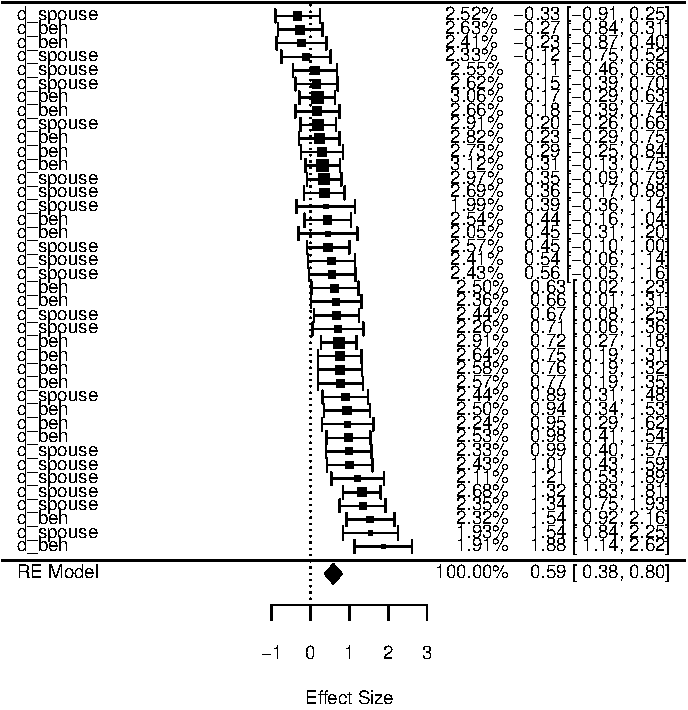
\includegraphics{Beck_HW_9_R_1_files/figure-latex/unnamed-chunk-6-1} \end{center}

\begin{Shaded}
\begin{Highlighting}[]
\NormalTok{dist <-}\StringTok{ }\NormalTok{metafor}\OperatorTok{::}\KeywordTok{ranef.rma.mv}\NormalTok{(fit2)[[}\DecValTok{1}\NormalTok{]] }\OperatorTok\StringTok{ }\NormalTok{data.frame }\OperatorTok
\StringTok{  }\KeywordTok{mutate}\NormalTok{(}\DataTypeTok{pi.lb =} \KeywordTok{coef}\NormalTok{(fit2) }\OperatorTok{+}\StringTok{ }\NormalTok{pi.lb, }
         \DataTypeTok{term =} \KeywordTok{rownames}\NormalTok{(.),}
         \DataTypeTok{sign =} \KeywordTok{sign}\NormalTok{(pi.lb)) }\OperatorTok
\StringTok{  }\KeywordTok{separate}\NormalTok{(term, }\KeywordTok{c}\NormalTok{(}\StringTok{"term"}\NormalTok{, }\StringTok{"scrap"}\NormalTok{), }\DataTypeTok{sep =} \StringTok{" [|] "}\NormalTok{) }\OperatorTok
\StringTok{  }\KeywordTok{group_by}\NormalTok{(term, sign) }\OperatorTok
\StringTok{  }\KeywordTok{summarize}\NormalTok{(}\DataTypeTok{n =} \KeywordTok{n}\NormalTok{())}
\end{Highlighting}
\end{Shaded}

12 of 20 of the spousal rating effect sizes differ from 0, while 12 of
20 of the behavior effect sizes differ from 0.

\subsection{Part B}\label{part-b-1}

Provide a funnel plot. Effect sizes outside the confidence region
suggest more heterogeneity than expected by sampling error. More effect
sizes on one side than the other suggest publication bias. Is there
evidence of either?

\begin{Shaded}
\begin{Highlighting}[]
\KeywordTok{funnel}\NormalTok{(fit2,}\DataTypeTok{addtau2=}\OtherTok{TRUE}\NormalTok{,}\DataTypeTok{xlab=}\StringTok{"Effect Size"}\NormalTok{,}\DataTypeTok{level=}\NormalTok{.}\DecValTok{95}\NormalTok{,}\DataTypeTok{back =} \StringTok{"grey"}\NormalTok{)}
\end{Highlighting}
\end{Shaded}

\begin{center}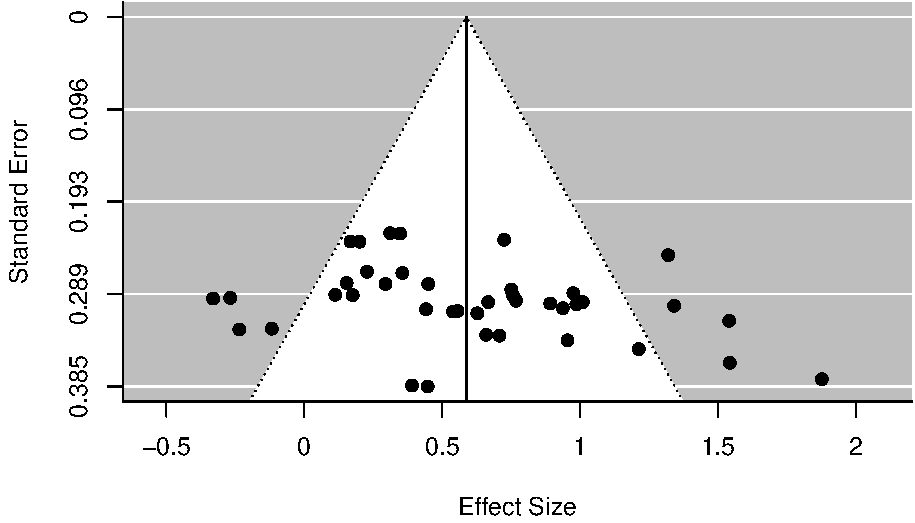
\includegraphics{Beck_HW_9_R_1_files/figure-latex/unnamed-chunk-7-1} \end{center}

The effect sizes in the funnel plot suggest that there is more
heterogeneity in the effect sizes than would be expected by sampling
error, which suggests we should look for moderators.

\section{Question 3}\label{question-3}

Now include the dummy codes for outcome type in a no intercept model.

\begin{Shaded}
\begin{Highlighting}[]
\NormalTok{fit3 <-}\StringTok{ }\KeywordTok{rma.mv}\NormalTok{(d, BD, }\DataTypeTok{mods =} \OperatorTok{~}\StringTok{ }\OperatorTok{-}\DecValTok{1} \OperatorTok{+}\StringTok{ }\NormalTok{d_b }\OperatorTok{+}\StringTok{ }\NormalTok{d_s, }\DataTypeTok{random =} \OperatorTok{~}\StringTok{ }\NormalTok{DV }\OperatorTok{|}\StringTok{ }\NormalTok{study, }\DataTypeTok{struct=}\StringTok{"UN"}\NormalTok{, }\DataTypeTok{data=}\NormalTok{New_Phobia_Data, }\DataTypeTok{tdist=}\OtherTok{TRUE}\NormalTok{, }\DataTypeTok{method=}\StringTok{"REML"}\NormalTok{)}
\KeywordTok{summary}\NormalTok{(fit3)}
\end{Highlighting}
\end{Shaded}

\begin{verbatim}
## 
## Multivariate Meta-Analysis Model (k = 40; method: REML)
## 
##   logLik  Deviance       AIC       BIC      AICc 
## -14.3971   28.7943   38.7943   46.9822   40.6693   
## 
## Variance Components:
## 
## outer factor: study (nlvls = 20)
## inner factor: DV    (nlvls = 2)
## 
##             estim    sqrt  k.lvl  fixed     level 
## tau^2.1    0.1431  0.3783     20     no     d_beh 
## tau^2.2    0.1542  0.3927     20     no  d_spouse 
## 
##           rho.d_bh  rho.d_sp    d_bh  d_sp 
## d_beh            1    0.8662       -    no 
## d_spouse    0.8662         1      20     - 
## 
## Test for Residual Heterogeneity:
## QE(df = 38) = 101.6060, p-val < .0001
## 
## Test of Moderators (coefficients 1:2):
## F(df1 = 2, df2 = 38) = 15.7487, p-val < .0001
## 
## Model Results:
## 
##      estimate      se    tval    pval   ci.lb   ci.ub 
## d_b    0.5807  0.1075  5.3995  <.0001  0.3630  0.7984  *** 
## d_s    0.5990  0.1102  5.4376  <.0001  0.3760  0.8220  *** 
## 
## ---
## Signif. codes:  0 '***' 0.001 '**' 0.01 '*' 0.05 '.' 0.1 ' ' 1
\end{verbatim}

\subsection{Part A}\label{part-a-2}

Was treatment effective in reducing the fear of spiders as measured by
the behvaioral measure?

According to the behavior reports, the treatment was effective in
reducing the fear of spiders, d = 0.58, 95\% CI {[}0.36, 0.8{]}.

\subsection{Part B}\label{part-b-2}

On average, how much better off was a treatment participant compared to
a control participant?

On average, an individual in the treatment group was able to move 0.58
SD closer to a tarantula than someone in a control group.

\subsection{Part C}\label{part-c-1}

Was treatment effective in reducing the fear of spiders as measured by
the spouce reports?

According to the spousal reports, the treatment was effective in
reducing the fear of spiders, d = 0.6, 95\% CI {[}0.38, 0.82{]}.

\subsection{Part D}\label{part-d-1}

On average, how much better off was a treatment participant compared to
a control participant?

\begin{Shaded}
\begin{Highlighting}[]
\NormalTok{V0=}\KeywordTok{matrix}\NormalTok{(}\KeywordTok{c}\NormalTok{(}\KeywordTok{c}\NormalTok{(.}\DecValTok{5}\NormalTok{, .}\DecValTok{5}\NormalTok{), }
            \KeywordTok{c}\NormalTok{(}\DecValTok{1}\NormalTok{,}\OperatorTok{-}\DecValTok{1}\NormalTok{)) , }\DataTypeTok{byrow =}\NormalTok{ T, }\DataTypeTok{nc =} \DecValTok{2}\NormalTok{)}
\KeywordTok{rownames}\NormalTok{(V0) <-}\StringTok{ }\KeywordTok{c}\NormalTok{(}\StringTok{"Behavioral + Spousal"}\NormalTok{, }\StringTok{"Behavioral v Spousal"}\NormalTok{)}
\NormalTok{glht_V0 <-}\StringTok{ }\KeywordTok{glht}\NormalTok{(fit3,}\DataTypeTok{linfct=}\NormalTok{V0,}\DataTypeTok{alternative=}\StringTok{"two.sided"}\NormalTok{,}\DataTypeTok{rhs=}\DecValTok{0}\NormalTok{)}
\NormalTok{res_V0    <-}\StringTok{ }\KeywordTok{confint}\NormalTok{(glht_V0, }\DataTypeTok{calpha =} \KeywordTok{univariate_calpha}\NormalTok{()) }
\NormalTok{res_V0_df <-}\StringTok{ }\NormalTok{res_V0}\OperatorTok{$}\NormalTok{confint }\OperatorTok\StringTok{ }\KeywordTok{data.frame}\NormalTok{()}
\end{Highlighting}
\end{Shaded}

On average, spouses reported individual in the treatment group were 0.59
SD (CI {[}0.38, 0.8{]}) less afraid than someone in the control group.

\subsection{Part E}\label{part-e}

Was the effect size for spouse reports significantly different from the
effect size for the behavioral measure?

There was no difference in effect size for spouse reports v. behavioral
measures, b = -0.02, 95\% CI {[}-0.13, 0.09{]}.

\subsection{Part F}\label{part-f}

How highly related are the true effect sizes for behavior and spouse
reports?

The true effect sizes are strongly correlated, r = 0.87.

\subsection{Part G}\label{part-g}

Examine the funnel plot for this model and comment on what has changed
compared to the unconditional model.

\begin{Shaded}
\begin{Highlighting}[]
\KeywordTok{par}\NormalTok{(}\DataTypeTok{mfrow =} \KeywordTok{c}\NormalTok{(}\DecValTok{1}\NormalTok{,}\DecValTok{2}\NormalTok{))}
\KeywordTok{funnel}\NormalTok{(fit2,}\DataTypeTok{addtau2=}\OtherTok{TRUE}\NormalTok{,}\DataTypeTok{xlab=}\StringTok{"Effect Size"}\NormalTok{,}\DataTypeTok{level=}\NormalTok{.}\DecValTok{95}\NormalTok{,}\DataTypeTok{back =} \StringTok{"grey"}\NormalTok{, }\DataTypeTok{xlim =} \KeywordTok{c}\NormalTok{(}\OperatorTok{-}\DecValTok{2}\NormalTok{,}\DecValTok{2}\NormalTok{), }\DataTypeTok{ylim =} \KeywordTok{c}\NormalTok{(}\DecValTok{0}\NormalTok{,.}\DecValTok{6}\NormalTok{))}
\KeywordTok{title}\NormalTok{(}\StringTok{"Model Q2"}\NormalTok{)}
\KeywordTok{funnel}\NormalTok{(fit3,}\DataTypeTok{addtau2=}\OtherTok{TRUE}\NormalTok{,}\DataTypeTok{xlab=}\StringTok{"Effect Size"}\NormalTok{,}\DataTypeTok{level=}\NormalTok{.}\DecValTok{95}\NormalTok{,}\DataTypeTok{back =} \StringTok{"grey"}\NormalTok{, }\DataTypeTok{xlim =} \KeywordTok{c}\NormalTok{(}\OperatorTok{-}\DecValTok{2}\NormalTok{,}\DecValTok{2}\NormalTok{), }\DataTypeTok{ylim =} \KeywordTok{c}\NormalTok{(}\DecValTok{0}\NormalTok{,.}\DecValTok{6}\NormalTok{))}
\KeywordTok{title}\NormalTok{(}\StringTok{"Model Q3"}\NormalTok{)}
\end{Highlighting}
\end{Shaded}

\begin{center}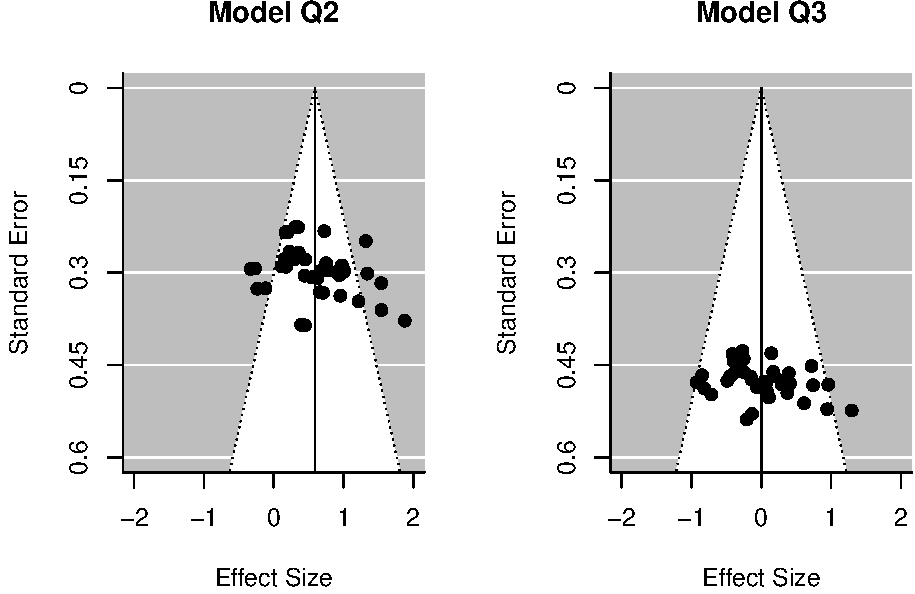
\includegraphics{Beck_HW_9_R_1_files/figure-latex/unnamed-chunk-10-1} \end{center}

The standard errors of the estimates are larger in the model that
estimates fixed effect effect sizes for both the behavioral and spousal
measures, but there is less heterogeneity, which suggests that adding in
the separate estimates improves model fit.

The funnel plot suggests \# Question 4\\
Now add the weeks of therapy variable as a moderator.

\begin{Shaded}
\begin{Highlighting}[]
\NormalTok{fit4 <-}\StringTok{ }\KeywordTok{rma.mv}\NormalTok{(d, BD, }\DataTypeTok{mods =} \OperatorTok{~}\StringTok{ }\OperatorTok{-}\DecValTok{1} \OperatorTok{+}\StringTok{ }\NormalTok{d_b }\OperatorTok{+}\StringTok{ }\NormalTok{d_s }\OperatorTok{+}\StringTok{ }\NormalTok{d_b}\OperatorTok{:}\NormalTok{weeks }\OperatorTok{+}\StringTok{ }\NormalTok{d_s}\OperatorTok{:}\NormalTok{weeks, }\DataTypeTok{random =} \OperatorTok{~}\StringTok{ }\NormalTok{DV }\OperatorTok{|}\StringTok{ }\NormalTok{study, }\DataTypeTok{struct=}\StringTok{"UN"}\NormalTok{, }\DataTypeTok{data=}\NormalTok{New_Phobia_Data, }\DataTypeTok{tdist=}\OtherTok{TRUE}\NormalTok{, }\DataTypeTok{method=}\StringTok{"REML"}\NormalTok{)}
\KeywordTok{summary}\NormalTok{(fit4)}
\end{Highlighting}
\end{Shaded}

\begin{verbatim}
## 
## Multivariate Meta-Analysis Model (k = 40; method: REML)
## 
##   logLik  Deviance       AIC       BIC      AICc 
##  -8.3482   16.6964   30.6964   41.7810   34.6964   
## 
## Variance Components:
## 
## outer factor: study (nlvls = 20)
## inner factor: DV    (nlvls = 2)
## 
##             estim    sqrt  k.lvl  fixed     level 
## tau^2.1    0.0369  0.1920     20     no     d_beh 
## tau^2.2    0.0806  0.2840     20     no  d_spouse 
## 
##           rho.d_bh  rho.d_sp    d_bh  d_sp 
## d_beh            1    0.6987       -    no 
## d_spouse    0.6987         1      20     - 
## 
## Test for Residual Heterogeneity:
## QE(df = 36) = 79.7613, p-val < .0001
## 
## Test of Moderators (coefficients 1:4):
## F(df1 = 4, df2 = 36) = 17.6399, p-val < .0001
## 
## Model Results:
## 
##            estimate      se     tval    pval    ci.lb   ci.ub 
## d_b         -0.2125  0.2044  -1.0400  0.3053  -0.6270  0.2019      
## d_s         -0.0704  0.2375  -0.2967  0.7684  -0.5521  0.4112      
## d_b:weeks    0.1393  0.0338   4.1206  0.0002   0.0708  0.2079  *** 
## d_s:weeks    0.1176  0.0391   3.0045  0.0048   0.0382  0.1969   ** 
## 
## ---
## Signif. codes:  0 '***' 0.001 '**' 0.01 '*' 0.05 '.' 0.1 ' ' 1
\end{verbatim}

\subsection{Part A}\label{part-a-3}

Was treatment more effective the longer that patients were in treatment?

\begin{Shaded}
\begin{Highlighting}[]
\NormalTok{k <-}\StringTok{ }\KeywordTok{matrix}\NormalTok{(}\KeywordTok{c}\NormalTok{(}\DecValTok{0}\NormalTok{,}\DecValTok{0}\NormalTok{,.}\DecValTok{5}\NormalTok{,.}\DecValTok{5}\NormalTok{), }\DataTypeTok{nrow =} \DecValTok{1}\NormalTok{)}
\KeywordTok{rownames}\NormalTok{(k) <-}\StringTok{ "weeks"}
\NormalTok{glht_4a <-}\StringTok{ }\KeywordTok{glht}\NormalTok{(fit4,}\DataTypeTok{linfct=}\NormalTok{k,}\DataTypeTok{alternative=}\StringTok{"two.sided"}\NormalTok{,}\DataTypeTok{rhs=}\DecValTok{0}\NormalTok{)}
\NormalTok{res_4a    <-}\StringTok{ }\KeywordTok{confint}\NormalTok{(glht_4a, }\DataTypeTok{calpha =} \KeywordTok{univariate_calpha}\NormalTok{()) }
\NormalTok{res_4a_df <-}\StringTok{ }\NormalTok{res_4a}\OperatorTok{$}\NormalTok{confint }\OperatorTok\StringTok{ }\KeywordTok{data.frame}\NormalTok{()}
\end{Highlighting}
\end{Shaded}

Treatments were more effective the longer patients were in treatment, b
= 0.13, 95\% CI {[}0.06, 0.2{]}.

\subsection{Part B}\label{part-b-3}

Did length of therapy have different effects on the behavioral and
spouse report effect sizes?

Yes, the length of treatment moderated effect sizes for both measures.
For both behavioral (b = 0.14, 95\% CI {[}0.07, 0.21{]}) and spousal (b
= 0.12, 95\% CI {[}0.04, 0.2{]}) reports, effect sizes of treatment
increased with longer study durations.

\subsection{Part C}\label{part-c-2}

Examine the funnel plot again. Any evidence of lingering heterogeneity
that might be modeled with the inclusion of additional predictors?

\begin{Shaded}
\begin{Highlighting}[]
\KeywordTok{par}\NormalTok{(}\DataTypeTok{mfrow =} \KeywordTok{c}\NormalTok{(}\DecValTok{1}\NormalTok{,}\DecValTok{1}\NormalTok{))}
\KeywordTok{funnel}\NormalTok{(fit4,}\DataTypeTok{addtau2=}\OtherTok{TRUE}\NormalTok{,}\DataTypeTok{xlab=}\StringTok{"Effect Size"}\NormalTok{,}\DataTypeTok{level=}\NormalTok{.}\DecValTok{95}\NormalTok{,}\DataTypeTok{back =} \StringTok{"grey"}\NormalTok{)}
\KeywordTok{title}\NormalTok{(}\StringTok{"Model Q4"}\NormalTok{)}
\end{Highlighting}
\end{Shaded}

\begin{center}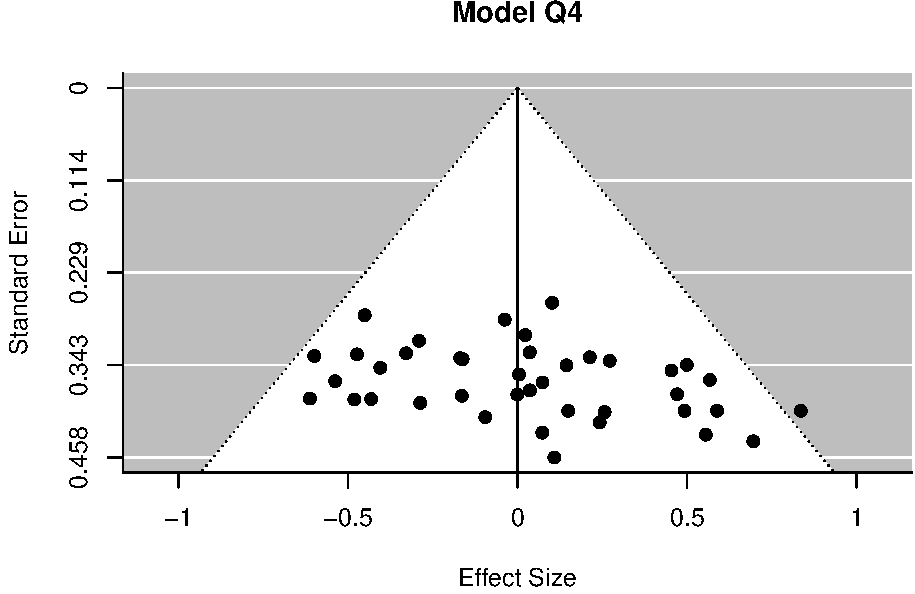
\includegraphics{Beck_HW_9_R_1_files/figure-latex/unnamed-chunk-13-1} \end{center}

There is only one study whose effect size falls outside of the bounds we
would expect


\end{document}
